

\newlength{\questlenght}
\settowidth{\questlenght}{\textbf{Question iii}\ \ }
\newlength{\textminusquest}
\setlength{\textminusquest}{\textwidth}
\addtolength{\textminusquest}{-\questlenght}
\newcommand{\ques}[2]{%
\noindent\textbf{Question #1}\hfill
\begin{minipage}[t][25pt][t]{\textminusquest}
    #2
\end{minipage}    
}


\chapter{Introduction}\label{chap:intro-english}


\begin{abstract}
    First of all, we present and motivate the research work carried out as part of this thesis. The aim is to improve
methods for seismic probabilistic risk assessment studies, given the lack of response provided by the state of the art regarding the choice of the prior in Bayesian inference. Secondly, we present the organization of the manuscript, which is based on a reformulation of the problematic under
in the form of six main questions.
\end{abstract}

\minitoc


\section{Motivation and positioning of the thesis}






\subsection{Probabilistic risk assessment studies}


\subsubsection{History}


Probabilistic risk assessment (PRA) studies refer to a set of technical analysis methods that allow for the quantification of the risks faced by a facility when exposed to a particular event. This event may be of natural or artificial origin (technological, human, etc.), and may stem from internal or external sources. It can take the form of an earthquake, a flood, a series of internal failures, among others.

Following the early recommendations of F. R. Farmer (a safety expert at the UK Atomic Energy Authority) in the 1960s concerning the reliability of nuclear facilities, these methods share a common feature: the incorporation of the notion of uncertainty into the characterization of the event, its phenomena, and its attributes (thus referred to as the ``hazard''). Their framework and concepts were quickly adopted and further developed in the United States (see the report by the Nuclear Regulatory Commission, \cite{nrc_pra_1983}). Notably, many studies began integrating seismic reliability analyses since 1968 \citep{cornell_engineering_1968}, thereby laying the groundwork for seismic probabilistic risk assessment (SPRA) studies.



Earthquakes indeed represent a significant risk factor in safety assessments. Firstly, although commonly characterized by their magnitude and distance from the source, seismic signals are far more complex than a simple bivariate function. Two earthquakes with the same magnitude and source can exhibit significantly different characteristics (and consequences). Secondly, because an earthquake can simultaneously affect all elements —--both external and internal—-- to a facility, it has the potential to cause severe damage to equipment and structures. The potential cost of the consequences of a seismic hazard can thus be high and critical in the nuclear context, making it an event of major and decisive importance, even in geographical areas where such events are rare.


Nowadays, accounting for seismic hazard within the framework of probabilistic risk assessments is an international recommendation in the context of the nuclear industry. In France, its application within that industry is defined by the nuclear safety and radiation protection authority (ASNR in French\footnote{Foremerly ASN: the nucelar safety authority (ASN) was unifed with the radioprotectection and nuclear safety institute (IRSN) in January 1, 2025.} ), as outlined in the fundamental safety rule \citep{asn_regle_2002}.



\subsubsection{The evolution of PRA in France, at the CEA, and in This Thesis}

The evolution of methods and knowledge related to the safety of nuclear installations progresses in parallel with changes in the regulations and standards imposed upon them. Concerning seismic hazard, the relationship between evolving rules and methods (and thus of PRA studies) brings into play differing perspectives, primarily between the main operator (EDF) and the experts of the safety authority (formerly the IRSN, now unified with the nuclear safety authority under the ASNR).
For the operator, the robustness of the installation should not be fundamentally questioned by advancements in knowledge or methodology, as uncertainties are already accounted for through safety margins incorporated during the equipment’s design. The authority’s experts, on the other hand, argue that robustness must be continuously reassessed, and that safety margins are not intended to be gradually consumed as knowledge advances \citep{roger_seisme_2020}. %improves 
In this dialogue, the ASNR acts as a kind of referee. Among other responsibilities, it defines the ``augmented safety earthquake'' (a conservative amplification of the ``maximum historically credible earthquake''), which serves as the reference margin in demonstrating an equipment's seismic robustness.



This arbitration is thus both sensitive and critical.
The incident that occurred in 2011 at the Fukushima-Daiichi nuclear power plant illustrates this clearly. The seismic hazard (which triggered the tsunami) had been underestimated by the consensus of Japanese experts, and it is ultimately this underestimation that led to the accident (see the report by the international atomic energy agency, \cite{iaea_fukushima_2015}). In the wake of this event,
 the ASNR decided to amplify the ``augmented safety earthquake'' by a factor of 1.5 in France\footnote{Defining in this respect the ``hard core earthquake''.}
 for the equipments that belong to the ``hard core'' (a limited list of systems, structures, and essential components to the upkeep of a nuclear installation).
 This led to require operators to provide an amplified demonstration of the robustness of their installations.

Within this context, the role of the CEA is ambivalent in the French nuclear landscape. On one hand, it operates research nuclear facilities and is therefore responsible for demonstrating the seismic robustness of its own equipment. On the other hand, it is also involved in collaborative research related to the civil nuclear fleet operated by EDF. A part of the research and expertise on the consequences of seismic hazards is carried out at the CEA’s EMSI laboratory, which is equipped with an experimental platform (called Tamaris). This facility enables mechanical testing of equipment under simulated seismic conditions.
Advancing methods for the SPRA framework is a focus area for the CEA that falls within the mission of this laboratory. As the CEA is accountable to safety authorities for its installations, it seeks to develop increasingly rigorous methods to justify their seismic performance.

This thesis fits into that process of evolving SPRA methodologies and reinforce safety demonstrations. Funded by the CEA as part of a research training grant, its aim is to enrich the state of the art in seismic fragility assessment for equipment and installations. The goal is to develop methods that are:
(i)~effective in the face of the complexity of both the studied systems and the hazard itself,
(ii)~robust over time and resilient to potential reevaluations of safety criteria, and
(iii)~transparent and auditable by safety authorities.


\subsection{Uncertainty quantification in probabilistic risk assessment studies}

% \subsubsection{}
\subsubsection{Principles and steps of uncertainty quantification}

Probabilistic risk assessment studies rely on the identification and quantification of uncertainties that arise during the evaluation of risk within a physical system. Uncertainty quantification is, in fact, a systematic process that aims at modeling and analyzing uncertainty, its sources, and how it propagates through the modeling of the studied physical system. This process lies at the intersection of physics, engineering, and applied mathematics, and has even emerged as a unique discipline  within the field of statistics.

It focuses on three key elements that describe the interaction between the physical system and the hazard: input parameters $\mbf X$, the physical response of the system $Y$, and a modeling of the latter: $Y = \cM(\mbf X)$.
This functional $\cM$ represents the (often complex) modeling of the system and its physical properties. This model may involve solving physical equations, running numerical simulations, or even analyzing the result of a mechanical experiment.
The general approach to uncertainty quantification typically consists into several key steps (see, for example, 
\cite{sudret_uncertainty_2007,iooss_contributions_2009}) that we detail below:
\begin{enumerate}
    \item Identification of uncertainty sources:
    It is common to classify uncertainties into two main categories. On one hand, irreducible uncertainties, which arise from the inherent and ``natural'' randomness embedded in the hazard and the physical system itself. On the other hand, epistemic uncertainties, which result from a lack of information and are therefore considered reducible, in contrast to the former \citep{hullermeier_aleatoric_2019}. This step leads to a probabilistic modeling of the input $\mbf X$.
    \item Uncertainty propagation: This step involves approximating the distribution of the model output $\cM(\mbf X)$, and evaluating a quantity of interest that depends on it, such as a variance, a failure probability, etc. More generally, this means evaluating a quantity of the form $\mathbb{E}\phi(Y)$.
    \item Sensitivity analysis: This step aims to provide insight into how uncertainties propagate through the system, by identifying the influence of one or more of the input parameters on the output $Y$ \citep{iooss_review_2015}.
\end{enumerate}

\subsubsection{Mathematical tools in uncertainty quantification}

Numerous mathematical tools support the aforementioned steps of uncertainty quantification. While this manuscript does not aim to provide an exhaustive overview of them, the following highlights several examples that are directly relevant to the work presented in this thesis:

\begin{itemize}
    \item Surrogate modeling helps to address the complexity involved in evaluating the model $\cM$, by constructing a surrogate model $\tilde{M}$, trained on a dataset of observations $(\mbf x_1, y_1), \ldots, (\mbf x_k, y_k)$. The surrogate model is, by design, simpler to evaluate than the original model. Its definition is not limited and its form can range from a simple parametric function to the output of a ``black-box'' neural network. Among the most commonly used approaches we can cite Gaussian processes (or kriging) and polynomial chaos expansions.
    \item Global sensitivity indices are a core component of the sensitivity analysis step. Since the early work of \citet{sobol_sensitivity_1993}, they have become essential tools for statistically measuring how the system output $Y$ is influenced by one or several of the input variables $X_i$ (where $\mbf X = (X_1, \ldots, X_p)$). In this context, the impact of input $X_i$ on $Y$, denoted $S_i$, is expressed as the expected divergence between the distribution $P_Y$ of $Y$ and its conditional distribution given $X_i$, $P_{Y|X_i}$ (Da Veiga, 2015):
\begin{equation}
    S_i = \mathbb{E}_{X_i}[D(P_Y \,||\, P_{Y|X_i})],
\end{equation}
    where $D$ is a dissimilarity measure between two probability distributions. The choice of $D$ is crucial in defining $S_i$. For instance, choosing $D(P||Q) = \| \mathbb{E}_{X \sim P}[X] - \mathbb{E}_{X \sim Q}[X] \|^2$ corresponds to a first-order Sobol’ index. The choice of $D$ can be driven by various considerations, such as the desire to detect independence between $X_i$ and $Y$. The next item explores a range of potential choices for $D$.
    \item  Information theory lies at the heart of comparing probability measures, and thus, of uncertainty quantification. By nature, the ways in which two distributions spread information over a space are numerous. In the definition of $S_i$ above, the selection of $D$ (and therefore the form of $S_i$) is inherently tied to information-theoretic principles.
    
      A widely used class of divergences, perceived as an extension of Shannon entropy, is the $f$-divergences class, introduced by \citet{csiszar_information-type_1967}. These divergences are used across many fields beyond sensitivity analysis, such as in variational inference \citep{minka_divergence_2005,bach_sum--squares_2023}, surrogate model design \citep{nguyen_surrogate_2009}, and PAC-Bayesian learning \citep{picard-weibel_change_2022}. When $f$ is convex and satisfies $f(1) = 0$, the $f$-divergence is defined as:
      \begin{equation}\label{eq:intro-english:Df}
      D_f(P||Q) = \int_\cX f\left(\frac{p(x)}{q(x)}\right) q(x) \, d\omega(x),
      \end{equation}
      where $p$ and $q$ are densities of $P$ and $Q$ with respect to a common base measure $\omega$ on their domain $\mathcal{X}$. Thus, $f$-divergences reduce the choice of $D$ to a choice of the function $f$. A commonly used subclass is the $\delta$-divergences class \citep{zhu_information_1995}, defined fixing $f=f_\delta$ where:
      \begin{equation}
        f_\delta(x) = \left\lbrace\begin{array}{l l} \frac{x^\delta-\delta x-(1-\delta)}{\delta(\delta-1)} & \text{if\ }\delta\not\in\{0,1\},\\ 
            x\log x-x+1  & \text{if\ }\delta=1, \\
            -\log x +x -1 & \text{if\ }\delta=0.
        \end{array}\right. 
    \end{equation} 
      Notably, the well-known Kullback-Leibler divergence (denoted KL) can be viewed as a special case of $\delta$-divergences. We recall that:
        \begin{equation}
            \text{KL}(Q||P) = \int \log\left(\frac{q(x)}{p(x)}\right) q(x) \, d\omega(x)
        \end{equation}
        (with the same notations as in \cref{eq:intro-english:Df}), so that:
        \begin{equation}
            D_{f_\delta}(P||Q) = \text{KL}(P||Q) \text{ if } \delta = 1, \quad D_{f_\delta}(P||Q) = \text{KL}(Q||P) \text{ if } \delta = 0.      
        \end{equation}
      Of course, many dissimilarity measures are not $f$-divergences. First-order Sobol’ indices, mentioned above, are one such example. Another notable example is the Maximum Mean Discrepancy (MMD). Let $P, Q$ be probability measures over a set $\mathcal{X}$, and let $\mathcal{H}$ be a reproducing kernel hilbert space (RKHS) over $\mathcal{X}$ with reproducing kernel $k : \mathcal{X} \times \mathcal{X} \to \mathbb{C}$. The MMD \citep{gretton_kernel_2012} is defined as:
        \begin{equation}
            \text{MMD}(\mathcal{H};\, P||Q) = \sup_{\substack{f \in \mathcal{H}\\ \|f\|_{\mathcal{H}} \leq 1}} |\mathbb{E}_{X \sim P}f(X) - \mathbb{E}_{X \sim Q}f(X)|,
        \end{equation}
      or more simply:
      \begin{equation}
        \text{MMD}^2(\mathcal{H};\, P||Q) = \mathbb{E}_{X, X' \sim P \otimes P}[k(X, X')] + \mathbb{E}_{Y, Y' \sim Q \otimes Q}[k(Y, Y')] - 2 \mathbb{E}_{X,Y \sim P\otimes Q}[k(X, Y)].
      \end{equation}

    \item Reproducing kernel Hilbert spaces, although not widely used in this thesis, represent a powerful tool for modeling and representing complex objects. Through the use of their 
    kernel, they enable the manipulation of non-linear objects in a Hilbert linear space. In the case of the
    MMD defined above, RKHSs are used to represent and compare probability measures.

    A RKHS consists in a given Hilbert space $\cH$, sub-space of a functional space $\cF=\{f:\cX\to\CC\}$, such that for any $x\in\cX$, the mapping $f\mapsto f(x)$ is continuous on $\cH$. Then, the reproducing kernel is the unique mapping $k:\cX\times\cX\to\CC$ such that for all $x\in\cX$, $f\in\cH$,
      \begin{equation}
        f(x) = \langle f,k(x,\cdot) \rangle_\cH,
      \end{equation}
    where $\langle\cdot,\cdot\rangle_\cH$ denotes the scalar product on $\cH$. Among other fundamental properties of the theory, Aronszajn's theorem \citep{aronszajn_theory_1950} states the existence of the an RKHS from a given kernel that is symetric and postitve definite on $\cX$. For an in-depht look to the theory, we invite the interested reader to refer to \cite{scholkopf_learning_2001}.

    \item  Bayesian analysis is a fundamental tool in uncertainty quantification, 
    as it fundamentally introduces a form of uncertainty
    % as it introduces a formal representation of uncertainty 
    in one or more parameters of the studied model. The uncertainty encoded in the Bayesian framework typically appears in the form of a prior distribution. Propagation of uncertainties within this framework is achieved by computing the posterior distribution, based on statistical observations $(\mbf x_1, y_1), \ldots, (\mbf x_k, y_k)$.
      The choice of the prior is critical: it belongs to the step of uncertainty identification and significantly influences the posterior. As such, in the context of probabilistic risk assessments, it directly affects safety evaluations.

      Bayesian analysis is whole paradigm. Since it is central to this thesis, the next section is fully dedicated to it.
\end{itemize}









\subsection{The choice of the prior in Bayesian studies}

Bayesian analysis is a branch of statistics built upon an interpretation of probability as a degree of plausibility of events, generally referred to as ``credibility''. Like any statistical method, it aims to establish a connection between observed data and their underlying probability distribution. It relies on Bayes’ theorem, treating the unknown parameter that define the data distribution as random. Statistical observations then inform the distribution of these unknow paramters, updating the credibility attributed to one possible distribution of the data over another.

By contrast, the frequentist approach views probability as a 
%long-run 
frequency of occurrence, observable through repeated experimentations. In this paradigm, the unknown quantity exists as a fixed value, and the frequencies observed through repeated trials are more or less probable depending on which value of the unknown we assume to be true. This leads to what is typically termed ``confidence''.

It is important to note that these two approaches are complementary %rather than contradictory**, 
and they often intersect, depending on the specific context. In practical applications, the nature of the case study and its particular constraints may lead to favoring one approach over the other.

This thesis focuses on Bayesian analysis within the context of statistical inference. Here, a variable of interest $Y \in \mathcal{Y}$ is modeled using a parametric distribution $P_{Y|\theta}$, where $\theta \in \Theta$ is the unknown parameter, now treated as a random variable under the Bayesian framework. Accordingly, $\theta$ is assigned a distribution known as the \textbf{prior}. When we observe successive and conditionally independent realizations of $Y$, the \textbf{posterior} is defined as the distribution of $\theta$ conditionally to those observations.
A credibility region at level $r$ is defined as a region within $\Theta$ that holds at least probability $r$ under the posterior distribution. We note that various results establish links between the Bayesian and frequentist approaches to estimating $\theta$. One such result is the Bernstein–von Mises theorem (see e.g. \cite{van_der_vaart_asymptotic_1992}), which shows convergence between the two perspectives under certain conditions.

Let $\mbf y = (y_1, \ldots, y_k)$ represent the observed values from $k$ realizations of $Y$. Assuming all necessary quantities are well-defined, let:
$\pi$ be the density of the prior (with respect to some measure $\nu$), $\ell(\cdot|\theta)$ be the density of $P_{Y|\theta}$ (with respect to a measure $\mu$),
and $\ell_k(\mbf y|\theta) = \prod_{i=1}^k \ell(y_i|\theta)$ be the likelihood of the model.
With these notations, Bayes’ theorem defines the posterior density (with respect to $\nu$) as:
\begin{equation}
    p(\theta|y) = \frac{\ell_k(y|\theta)\pi(\theta)}{\int_\Theta \ell_k(y|\theta)\pi(\theta) \, d\nu(\theta)}.
\end{equation}
This formula formalizes the link between the prior, the model (represented via the likelihood), the data, and the posterior, which ultimately reflects the updated, credible prediction. It illustrates the Bayesian framework as an information transmission chain leading to the \emph{a posteriori}, from  two sources: the ``real''  (the observations) and the \emph{a priori}. This structure is illustrated in the diagram below.
\begin{figure}[h]
    \centering
    \begin{tikzpicture}

        \draw[-{Latex[length=1.5mm]}] (0, 0) -- (.9, 0); % english (0, 0) -- (.9, 0); 
        \draw (0, 0) node[left] {Dataset $\mbf y=(y_i)_{i=1}^k\in\cY^k$}; %english (0,0)
         
        \draw (2.5, 0) node {likelihood ${\ell_k(\mbf y|\theta)}$}; %englih (2.5,0)
        
        \draw[-{Latex[length=1.5mm]}] (0, -0.6) -- (0.9, -0.6); % english (0, -0.6) -- (0.9, -0.6); 
        \draw (0,-0.6) node[left] {Parameter $\theta\in\Theta$}; %english (0,-0.6)
        
        \draw (2.5,-0.6) node {prior $\pi(\theta)$}; % english (2.5,-0.6)

        \draw [-] plot [smooth] coordinates {(4.3,0) (4.6,-0.03) (5.05,-0.27) (5.5,-0.3)};
        \draw [-{Latex[length=1.5mm]}] plot [smooth] coordinates {(4.3,-0.6) (4.6,-0.57) (5.05,-0.33) (5.5,-0.3)};

        \draw (5.7,-0.3) node[right] {posterior $p(\theta|\mbf y)\propto{\ell_k(\mbf y|\theta)}{\pi(\theta)}$};
        
    \end{tikzpicture}
\end{figure}

If the information provided by the data is generally not questionned, it is the prior information that captures the most attention. By nature, the prior is the source of uncertainty in the result. Thus, its construction must be handled with care during the modeling stage and cannot be arbitrary. Yet the Bayesian formulation 
let it significantly influence   the posterior, especially in situations where the dataset is limited in size. 
An illustration of this phenomenon is proposed \cref{fig:intro-english:intro-differentsposteriors}, where different priors —--that seem similar—-- lead to very different posteriors, all based on the same observations. As always, the devil is in the detail: here, it is the tails of the prior distributions —--barely visible in the figure—-- that account for the discrepancy. Still, this example rightly raises concerns about the choice of prior.


\begin{figure}[h]
    \centering
    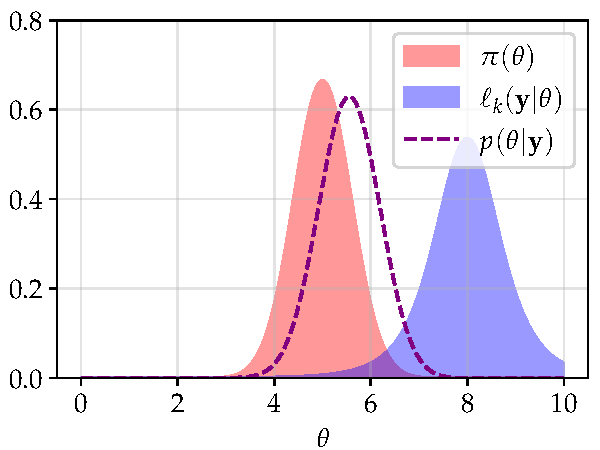
\includegraphics[width=5cm]{figures/intro/posterior1.pdf}
    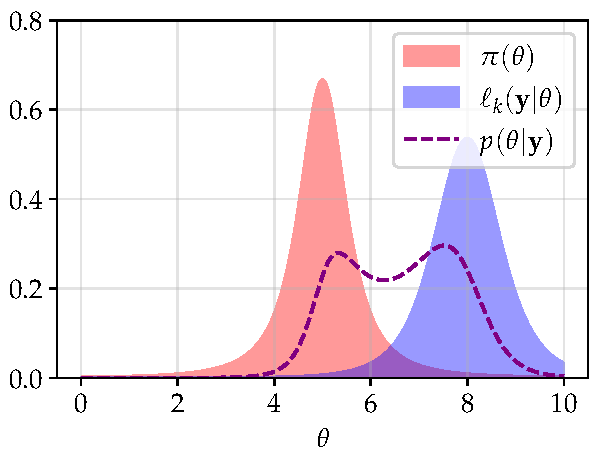
\includegraphics[width=5cm]{figures/intro/posterior2.pdf}
    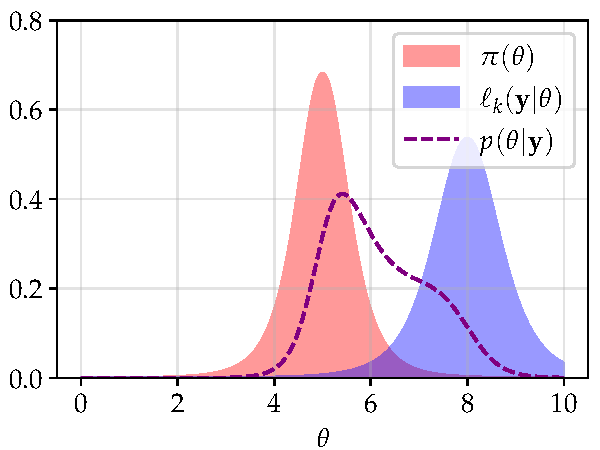
\includegraphics[width=5cm]{figures/intro/posterior3.pdf}   
    \caption{Different posteriors (dashed lines) derived from the same likelihood (blue) but different priors (red).%De gauche à droite le prior est : une gaussienne $\cN(5,)}
    }
    \label{fig:intro-english:intro-differentsposteriors}
\end{figure}

The question of how to construct a prior remains an open issue in the literature. For some, it is an opportunity to incorporate information from external sources, such as expert judgment, historical data, or known properties expected of the result. Such priors are typically described as informative. For others, the prior is instead a way for injecting uncertainty into the model. In other term, a way of expressing a lack of prior knowledge and allowing the data to speak for themselves. These practitioners place their trust in the modeling of the likelihood and their prior will be qualified as non-informative.

What emerges from these introductory paragraphs is that the question is unsolvable: there can be no universally accepted method for selecting a prior. This issue represents one of the ``holes'' in the Bayesian workflow identified by \citet{gelman_holes_2020}: overly informative priors can undermine confidence in the results, while excessively vague priors can lead to credibility regions so wide they become impractical. That said, this does not diminish the relevance of the Bayesian approach, this section is not intended to discredit it, and the remainder of the manuscript will prove that. But it must leave the one who use it aware of the impact and limitations of their choices. The selection of a prior is as critical as the choice of the model itself.











\subsection{What motivates research on prior elicitation for SPRA studies}

Bayesian analysis has become increasingly popular across many fields, including reliability and safety studies. Indeed, it is widely appreciated for its ability (i)~to introduce and propagate uncertainty in an inference problem, and (ii)~to exhibit more regular behavior than many frequentist methods, particularly when the number of observed data is limited.

The Bayesian inference framework naturally aligns with the  uncertainty quantification process. Identifying uncertainties in the input $\mbf X$ or within the model $\cM$ itself (or a surrogate, when applicable) can be achieved through their parameterization, resulting in a parametric distribution of the output $Y$: $P_{Y|X,\theta}$. The variable $\theta$, which is treated as random under the Bayesian paradigm, can represent various sources of uncertainty, differing in nature depending on the context \citep{bousquet_contributions_2024}. This approach has been widely employed across a range of models, including Gaussian processes (e.g., \cite{gu_parallel_2016}) and neural networks \citep{arbel_bayes_2023}.

Sometimes, the methodology is adopted specifically for the flexibility it offers in incorporating expert judgment or prior knowledge. Yet, it is this possibility that also questions, as it introduces a degree of subjectivity that is often difficult to justify. In the context of SPRA in the nuclear industry, demonstrating robustness is essential. Given the high complexity of such case studies, 
one xould find as many priors as there are experts if we follow this approach.
Such a caricatural situation puts at risk the auditability of any resulting posterior credibility region.

It becomes clear that in an auditable safety study, a ``good'' credibility region for an estimated parameter is not necessarily a narrow one, even if it seems to suggest that safety is achieved. Conversely, a region that is too wide is not inherently ``good'' either, as it fails to demonstrate the expected robustness of the equipment. The appropriate balance is complex, and the ``right'' prior is the one that produces results that inspire trust, while accurately reflecting the equipment’s ability or inability to handle the hazard.

All these reflections highlight the importance of constructing the prior in a methodical and disciplined way within the context of SPRA, using a rigorous framework that seeks, as much as possible, to avoid the introduction of any form of subjectivity into the process.





\section{Outline of the manuscript and contributions}

\subsection{Problem statement and organization of the thesis}



Several central questions emerge from this introduction and the preceding reflections. They are listed below and represent the major issues that arose during this thesis, which the work presented in this manuscript aims to address.\\

\ques{i}{How can one define and support the objectivity of a prior?}


\ques{ii}{What are the limitations of implementing such non-informative priors, and how can their use be reconciled  with practical needs?}

\ques{iii}{How can such priors be constructed and derived in practice?}

\ques{iv}{In the context of SPRA, what forms do these objective priors take within a seismic fragility curve model?}

\ques{v}{What are the implications of information scarcity in such models, and how can they be addressed?}

\ques{vi}{How can the different sources of information (\emph{a priori} information and data-based information) be best integrated across the full Bayesian workflow of the model under study?}\\[1pt]


In this thesis, we aim to address these six questions through a study structured along two axes.
The first axis is theoretical in nature and tackles the issues surrounding the construction of so-called ``objective'' priors. It focuses on the development of a theoretical framework known as reference prior theory.
The second axis is more practical, examining the application of the theoretical developments to real-world case studies. It focuses  on the estimation of seismic fragility curves, which are a key tool in the framework of seismic probabilistic risk assessment studies.
It is important to emphasize that, although distinct, these two major axes of work are deeply interconnected. Practical concerns inspired the theoretical investigations, just as theoretical insights have been applied to serve practical studies.\\



The \cref{part:ref-theory} of this manuscript is devoted to the development of the reference prior theory.

\noindent
In \cref{chap:intro-ref}, the theory is introduced and its state of the art is reviewed. This chapter presents the notion of reference prior as it is commonly defined in the literature and situates it within the objective priors. This chapter allows to formalize the mathematical framework that will be used throughout the rest of this part.

\noindent
In \cref{chap:ref-generalized}, we observe that the definition of reference priors relies on a dissimilarity measure. The chapter seeks to generalize this measure in order to reinforce the objectivity of reference priors. This work provides an answer to \textbf{question i}.

\noindent
In \cref{chap:constrained-prior}, the theory is extended to address the practical challenges that arise when reference priors, are difficult to use. The chapter introduces the concept of constrained reference priors, whose solutions propose an answer to \textbf{question ii}.

\noindent
In \cref{chap:varp}, a numerical method is developed to approximate reference priors. This method is based on variational inference, defining the prior as the output of a neural network in order to avoid an explicit calculation. This chapter provides an answer to \textbf{question iii}.\\


The \cref{part:spra}
of this manuscript address the topic of objective Bayesian estimation of seismic fragility curves.

\noindent
In \cref{chap:frags-intro}, seismic fragility curves are introduced along with their definition, historical background, and role within the SPRA. A review of the main estimation methods, based on the types of available data, is presented.

\noindent
In \cref{chap:prem}, a detailed computation and study of the reference prior is carried out for a classical model used to estimate fragility curves. Bayesian inference using this prior is then compared to other methods. This chapter addresses \textbf{question iv}.

\noindent
In \cref{chap:constrained-frags}, the limitations of the model used for fragility curve estimation are taken into account. A solution is proposed, supported by the theoretical developments from the first part. This chapter proposes an answer to \textbf{question v}.

\noindent
In \cref{chap:doe}, the study is concluded with a method designed to enhance Bayesian estimation, not only by optimizing the prior selection, but also by improving data selection itself through an experimental design strategy. This chapter provides an answer to \textbf{question vi}.\\

A general conclusion ends the manuscript in the final \cref{part:conclusion}.



\subsection{List of contributions}


The research conducted through this thesis led to the production of several contributions to the scientific litterature. Hereafter are listed the published and submitted works.



\subsubsection{Journal papers}



\begin{itemize}
    \item \textbf{A. Van Biesbroeck}, C. Gauchy, C. Feau \& J. Garnier (2025). ``Robust a posteriori estimation of probit-lognormal seismic fragility curves via sequential design of experiments and constrained reference prior''. \emph{arXiv} 2503.07343. \textsc{doi:} \href{https://dx.doi.org/10.48550/arXiv.2503.07343}{10.48550/arXiv.2503.07343}.
    \item N. Baillie, \textbf{A. Van Biesbroeck} \& C. Gauchy (2025). ``Variational inference for approximate reference priors using neural networks''. \emph{arXiv} 2502.02364. \textsc{doi:} \href{https://dx.doi.org/10.48550/arXiv.2502.02364}{10.48550/arXiv.2502.02364}
    \item \textbf{A. Van Biesbroeck} (2024). ``Properly constrained reference priors decay rates for efficient and robust posterior inference'', \emph{arXiv} 2409.13041. \textsc{doi:} \href{https://dx.doi.org/10.48550/arXiv.2409.13041}{10.48550/arXiv.2409.13041}
    \item \textbf{A. Van Biesbroeck}, C. Gauchy, C. Feau \& J. Garnier (2025). ``Design of experiments based on a low fidelity model for seismic fragility curves estimation''. \emph{ESAIM: ProcS} (to appear). \textsc{hal:} \href{https://hal.science/hal-04719458v1}{hal-04719458v1}
    \item \textbf{A. Van Biesbroeck} (2023). ``Generalized mutual information and their reference priors under Csizar f-divergence''. \emph{arXiv} 2310.10530. \textsc{doi:} \href{https://dx.doi.org/10.48550/arXiv.2310.10530}{10.48550/arXiv.2310.10530}
    \item \textbf{A. Van Biesbroeck}, C. Gauchy, C. Feau \& J. Garnier (2024). ``Reference prior for Bayesian estimation of seismic fragility curves''. \emph{Probabilistic Engineering Mechanics}, 76, pp 103622. \textsc{doi:} \href{https://dx.doi.org/10.1016/j.probengmech.2024.103622}{10.1016/j.probengm\-ech.2024.103622}
\end{itemize}






\subsubsection{Proceedings papers}



\begin{itemize}
    \item \textbf{A. Van Biesbroeck}, C. Feau \& J. Garnier (2025). ``Design of experiments for efficient and conform Bayesian learning of seismic fragility curves''. \emph{Proceedings of the 28th conference on Structural Mechanics in Reactor Techology (SMiRT).}
    \item N. Baillie, \textbf{A. Van Biesbroeck}, C. Feau \& C. Gauchy (2025). ``Bayesian estimation of seismic fragility curves based on variational reference priors using neural networks''. \emph{Proceedings of the 6th Thematic Conference on Uncertainty Quantification in Computational Sciences and Engineering (UNCECOMP)}.
    % \item C. Gauchy, \textbf{A. Van Biesbroeck}, C. Feau \& J. Garnier (2023). ``Inférence variationelle de lois a priori de référence''. \emph{Proceedings des 54èmes Journées de Statistiques (JdS)}. \textsc{url}
    \item \textbf{A. Van Biesbroeck}, C. Gauchy, J. Garnier \& C. Feau (2023). ``Connections between reference prior theory and global sensitivity analysis, an illustration with f-divergences''. \emph{Proceedings des 54èmes Journées de Statistiques (JdS)}. \textsc{hal:} \href{https://hal.science/hal-04171446}{hal-04171446}
    \item \textbf{A. Van Biesbroeck}, C. Gauchy, C. Feau \& J. Garnier (2023). ``Influence of the choice of the seismic intensity measure on fragility curves estimation in a Bayesian framework based on reference prior''. \emph{Proceedings of the 5th Thematic Conference on Uncertainty Quantification in Computational Sciences and Engineering (UNCECOMP)}, pp. 94-111. \textsc{doi:} \href{https://dx.doi.org/10.7712/120223.10327.19899}{10.7712/120223.10327.19899}
\end{itemize}




Each of these publications, whether it takes the form of a journal paper or a proceedings paper, proposes an original contribution that is tied to this thesis.
Naturally, the contributions presented as journal papers are considered as richer.

Apart from two exceptions, each of these contributions lies in the center of a chapter or an appendix of this manuscript.
The first exception is the proceedings paper published at JdS in 2023. Indeed, this work constituted an introduction to the study that led to the journal paper entitled ``Generalized mutual information and their reference priors under Csizar f-divergence''. In this manuscript, the proceedings paper is incorporated into the chapter tied with the latter (\cref{chap:ref-generalized}). The second exception is the proceedings paper published at SMiRT in 2025. The original methodology presented in this paper remains conceptual, and its development faced the end of  the thesis.
The study thus lacks for an in-depht examination that might be conducted in the future.






\chapter{Introduction en français}\label{chap:intro-french}

\renewcommand{\chaptertitlenamelng}{Chapitre}
\renewcommand{\partname}{Partie}


\begin{abstract}[Résumé]
    Ce chapitre ne diffère du \hyperref[chap:intro-english]{chapitre 1} que par sa rédaction en langue française.
    En premier lieu, nous introduisons et motivons les travaux de recherche qui ont été menés au cours de cette thèse. Ils s’inscrivent dans une problématique qui vise à améliorer les méthodes d’études sismiques probabilistes du fait du manque de réponse qu’apporte l’état de l’art à la question du choix du prior en inférence bayésienne. En second lieu, nous présentons l’organisation du manuscrit qui s’appuie sur une reformulation de la problématique sous la forme de six principales questions.
    %Dans ce chapitre, nous introduisons et motivons les travaux de recherche qui ont été conduits au cours de cette thèse. Les travaux sont motivés principalement par le besoin d'évolution des méthodes d'études sismiques probabilistes de sûreté, mais aussi par le manque de réponse qu'apporte l'état de l'art à la question du choix du prior en inférence bayésienne. Ces problématiques sont détaillées et les travaux sont alors introduits comme s'inscrivant dans celles-ci, le tout donnant lieu à une organisation consistante du manuscrit.
    %en introduisant à la fois leur inscription dans le cadre des études sismiques probabilistes de sûreté et dans le
    %
    %D'une part, nous introduisons le cadre des études sismiques probabilistes de dûreté, et 
    % Dans ce chapitre, nous mettons en lumière les différentes problématiques, à la fois issue de qui motivent 
    % Dans ce chapitre, nous introduisons les différents contextes qui motivent l'existence de cette thèse. D
\end{abstract}

\minitoc

\section{Motivation et positionnement de la thèse}

\subsection{Etudes probabilistes de sûreté}
%

\subsubsection{Historique}

Les études probabilistes de sûreté (EPS) désignent un ensemble de méthodes d'analyses techniques qui permettent de quantifier un risque encouru par une installation lorsqu'elle est sujette à un événement. L'événement peut être d'origine naturelle comme artificielle (technologique, humaine, etc), il peut être de provenance interne comme externe ; il peut s'agir d'un séisme, d'une inondation, d'une combinaison de défaillances internes, entre autres.  % (qui peut être d'origine naturelle comme artificielle, qui peut être interne comme externe). 

Faisant suite au premières recommandations de F. R. Farmer (expert sûreté à la UK atomic authority) dans les années 1960 pour la fiabilité des installations nucléaires,
ces méthodes ont pour caractéristique commune l'introduction de la notion d'incertitude dans la qualification de l'événement, ses phénomènes et ses caractéristiques (on parle alors d'aléa).
%
%Elles ont été introduites par F. R. Farmer dans les années 1960 [], qui plébiscitait cette idée d'étudier la fiabilité des installations nucléaires en prenant en compte l'aspect probabiliste et incertain des évenements auqelles elle est sujette.
%
Leur cadre et leur concept ont été rapidement adoptés et développés aux Etats-Unis (cf. le rapport de la Nuclear Regulatory Commission, \cite{nrc_pra_1983}). En particulier, de nombreuses études sont venues dès 1968 (\cite{cornell_engineering_1968}) 
y inscrire les analyses de fiabilité parasismique, définissant alors le cadre des études sismiques probabilistes de sûreté (SPRA en anglais). %, en particulier en ce qui concerne le cadre de la fiabilité parasismque.



Le séisme représente en effet un facteur de risque remarquable des études de sûreté.
Premièrement, bien que communément caractérisé par sa magnitude et sa distance à la source, son signal est bien plus riche qu'une fonction bivariée et deux séismes de même magnitude et de même source peuvent avoir des caractéristiques (et des conséquences) significativement différentes.
Deuxièmement, puisqu'il touche à la fois tous les éléments aussi bien externes qu'internes à l'installation, il est la potentielle source de conséquences lourdes sur les équipements et structures.
%voir de réactions en chaîne 
%qui atteindraient le ``noyau dur'' de l'installation (défini comme un ensemble d'élements critiques à l'installation). %, impliquant ainsi un coût élevé.
Le coût potentiel des conséquences d'un aléa sismique peut alors être élevé et critique dans le contexte nucléaire, ce qui en fait un événement d'intérêt majeur et décisif même dans les zones géographiques où il est rare.


%La prise en compte du séisme comme un aléa s'est confronté à la

Aujourd'hui, la prise en compte de l'aléa sismique sous le cadre des études probabilistes de sûreté est une recommandation internationale dans le contexte de l'industrie nucléaire. Leur cadre d'application dans l'industrie nucléaire française est précisé par l'autorité de sûreté nucléaire et de radioprotection (ASNR)\footnote{Anciennement ASN: l'autorité de sûreté nucléaire (ASN), a été unifiée avec l'institut de radioprotection et de sûreté nucléaire (IRSN) le 1\textsuperscript{er} janvier 2025.} dans la règle fondamentale de sûreté (\cite{asn_regle_2002}).









\subsubsection{L'évolution des EPS en France, au CEA, et dans cette thèse}



%Le rôle des études de sûreté d'une manière générale est de produire une quantification du risque d'une installation, d'une marge de fiabilité, et de démontrer son repsect d'un seuil défini par une autorité de régulation.
% Deux visions s'oppose relativement au sujet de l'avolution des méthodes et des conaissances relatives aux études de sûreté.
%Lors de la mise en place de de seuil et de la règle, plusieur point de vue, motivés par plusieurs intérêts peuvent alors se heurter. Il y a d'une part les exploitants, pour qui la notion de robustesse perdure d'elle même, les marges prises sont là pour tenir compte du manque de conaissances, et il y a ceux pour lesquels la robustess est sans cesse remise en question par les avancées des méthodes et des connaissances (\cite{roger_seisme_2020}).



%L'évolutions des méthodes et des conaissances relatives à la sûreté de 
L'évolution des méthodes et des connaissances relatives à la sûreté des installations nucléaires se fait de manière parallèle à l'évolution de la règle et de la norme imposées à celles-ci. 
Sur le sujet de l'aléa sismique, le rapport à l'évolution de la règle et de la méthode (et donc des EPS) oppose différents points de vue, principalement entre le principal exploitant (EDF) et les experts de l'autorité de sûreté (anciennement l'IRSN, maintenant unifié avec l'autorité de sûreté nucléaire devenue l'ASNR). 
Pour le premier, la robustesse de l'installation n'est normalement pas remise en question par l'avancée des connaissances et des méthodes puisque l’incertitude sur celles-ci fait parti des marges prises en comptes à la construction de l'équipement. %et calculées pour. 
Le second pense au contraire que la robustesse est une question perpétuelle et que la marge n’est pas faite pour être mordue au fil des connaissances qui s’ajoutent (\cite{roger_seisme_2020}). 
% L'évolution des méthodes EPS reste un champ de voies ouverte, pour lequel les approches s'opposent fondamentalement.
%Il est complxe de définir une voie d'évolution des EPS, et il n'y a pas de vision qui fait l'unanimté
L'ASNR se place alors en arbitre dans ce dialogue, entre autre elle définit le ``séisme majoré de sécurité''\footnote{Aujourd'hui plutôt appelé ``séisme de dimensionnement''.} (il s'agit d'une majoration du spectre du ``séisme maximal historiquement vraisemblable'' qui est définit par les sismologues) qui produit la marge de référence dans la démonstration de robustesse parasismique d'un équipement. % la marge de fiablité et séisme maximal à prendre en compte. %En ce qui concerne l'aléa sismique, le dialogue 
%
%Un tel dialogue n'est pas propre à la France, et 


Cet arbitrage est donc à la fois sensible et critique.
L'incident survenu en 2011 à la centrale nucléaire de Fukushima-Daiichi le démontre. L'aléa sismique (qui est la cause du tsunami) de référence
%fixé par le concensus des experts japonais
a été sous-évalué par le consensus des experts japonais, et c'est cette sous-évaluation qui est au final la cause de l'incident (cf. le rapport de l'agence internationale de l'énergie atomique, \cite{iaea_fukushima_2015}).
%En 2011, a eu lieu un incident 
Suite à cet événement, l'ASNR a pris la décision de majorer d'un facteur 1.5 le séisme majoré de sécurité\footnote{Définissant alors le ``séisme noyau dur''.} en France pour les équipements du ``noyau dur'' (liste limitée de systèmes, structures et composants essentiels au maintien des fonctions de sûreté d'une installation nucléaire). Ceci imposant alors une démonstration amplifiée de la robustesse des différentes installations par leur exploitant.



%valable pour certains éléments de l'installation faisant partie de ce que l'on appelle le "noyau dur" (liste limitée de systèmes, structures et composants essentiels au maintien des fonctions de sûreté des installations nucléaires)


%En 2011, à la suite de l'incident à la centrale de Fukushima suite au séisme survenu au large des côtes japonaises, ce dialogue s'est conclut par une imposition de la part de l'autorité de sûreté d'une majoration d'un facteur de 1.5 de ce séisme majoré de sécurité en France. % de la marge de fiabilité sismique des équipements nucléaires en France. 

%Devant le coût induit par 

%Cette différence démontre de la complexité du sujet






% Le séisme ne fait pas exception
% la place des EPS simsique dans cette différence de vision est très marquée puisque l'aléa du séisme reste une quesiton ouverte en soi, la moindre différence de choix de séisme maximim possible peut donner lieu à une ampleur de changement d'un coût très élevé pour l'exploitant



%Les études probabilistes de sureté ont été adoptées progressivement en France 


%En France, l'industrie nucléaire est réduite à un nombre restreint d'acteurs, exploitants, experts indépendants, et autorité.

% Ambivalence de la robustesse, deux notions 
% deux visions
% Le CEA, à la fois exploitatn et expert

Dans ce cadre, la place du CEA est ambivalente dans l'échiquier nucléaire français.
D'une part, il est exploitant d'install\-ations nucléaires de recherche 
et joue alors son propre rôle quant à la démonstration de robustesse de ses équipements.
% Aussi,
%, et ausi %titulaire d'une mission d'expertise de sûreté.
% il participe à l'expertise conjointe des expertises de sûreté relatives au parc nucléaire civil exploité par EDF. 
Aussi, il participe conjointement à des actions de recherche relatives au parc nucléaire civil exploité par EDF.
%Le CEA joue son propre rôle dans l'évolution de la démonstration de la robustesse de ses propres equipements et installations. 
Une partie de la recherche et l'expertise sur les conséquences de l'aléa sismique % études simqiques de sûreté au CEA 
se fait au CEA au laboratoire EMSI, qui dispose d'une plateforme expérimentale (Tamaris) qui permet de procéder à divers tests mécaniques sur des équipements sous séismes. 
%Le laboratoire d'etudes mécaniques et sismiques (EMSI) s'inscrit pleinenemnt dans cette ambivalence. Propriétaire de la plateforme d'expérimentation sismique Tamaris, le labortoire se place souvent au centre des études de fiabilité sismique et du dialogue entre EDF et les experts de l'ASNR.
L'approfondissement des méthodes des études sismiques probabilistes de sûreté est un enjeu pour le CEA qui s'inscrit dans les missions de ce laboratoire. Le CEA étant responsable devant les autorités de sûreté de ses installations, %il cherche %alors 
%à développer des méthodes toujours rigoureuses devant leur vieillissement. %de ces installations et de leurs équipements.
il cherche à développer des méthodes toujours rigoureuses pour justifier de leur tenue sismique.


% Le rôle du CEA est ambivalent dans cete equation, à la fois exploitant instut de recherche.
% Le CEA joue son propre rôle dans l'évolutions de la démonstration de robstesse de ses propres installations. Aussi il participe à l'expertise conjointe de méthodes d'EPS avec EDF.


% Le CEA est lui même exploitant, d'unstallations de recherche.
% Il a 

% L'evolutio des EPS y est toujours un enjeux pour être capable de produire une étude plus efficace, et des résultats plus convaincants aurpès des autorités.
% Le CEA est responsable auprès des autorités concernant ses installations et cherche à développer des méthodes toujours rigoureuses devant le vieillissemnt des installations

% Sur le sujet de l'aléa sismique, la démonstration de robustesse reste complexe vis à vis de la complexité de l'aléa lui-même, et de sa fréquence.
% Les EPS sont en constantes ré-évaluation à la demande des autorités de sûreté sur cette aspect, principalement depuis l'accident sur la centrale de Fukushima en 2011. %%% Peut etre mettre ca plus haut

% Au CEA, la recherche sur les études sismiques probabilistes de sûerté est portée par le laboratoire EMSI, qui dispose d'une plateforme experimentale (Tamaris) qui permet de procéeder à divers tests mécaniques sur des équipements sous séismes. 

Cette thèse s'inscrit dans la démarche d'évolution du SPRA et de démonstration de sûreté. Financée par le CEA dans le cadre d'un contrat de formation par la recherche, elle a pour objectif d'étoffer l'état de l'art en terme d'estimation de la fragilité sismique des équipements et des installations.
L'objectif est de développer des méthodes qui doivent le plus possible être (i) efficaces devant la complexité des objets étudiés et de l'aléa, (ii) être robustes dans le temps et devant une potentielle réévaluation des critères de sûreté, et (iii) être transparentes et auditables par les autorités de sûreté.

%lieu à des méthodes qui savent être efficace devant la complexité technique représentée efficaces devant la c

%en cherchant un cadre plus robuste, plus efficace.
%%%% Principalement en appuyant l'étude bayésienne de celles-ci.




\subsection{La quantification d'incertitudes dans les études probabilistes de sûreté} % la quantification d'incertitutde dans les EPS


\subsubsection{Principe et étapes de la quantification d'incertitudes}

%Le cadre des EPS regroupe un certains nmb
%Différents outils mathématiques sont employés dans le cadre des EPS et composent

Les études probabilistes de sûreté %et plus généralement les études probabilistes de fiabilité, de robustesse, et de  %les procédés de génie probabiliste d'études de fiabilité, de robustesse, et de 
s'appuient sur la 
prise en compte et la quantification des incertitudes qui apparaissent dans le procédé d'évaluation d'un risque au sein d'un système physique.
%lors de l'évaluation d'une quantité décrivant un risque. %d'un 
%
La quantification d'incertitudes représente en fait une démarche qui consiste à modéliser et analyser méthodiquement l'incertitude, sa source, et sa propagation au sein de la modélisation du système physique étudié. %étudié. %système phyisique?
Elle se construit alors à l'intersection de la physique, de l'ingénierie et des mathématiques appliquées, et s'érige même comme une branche des statistiques à part entière.

Elle concentre son étude sur 3 éléments qui décrivent l'interaction entre le système physique et l'aléa~: des paramètres d'entrée $\mbf X$, une réponse physique du système $ Y$, et une modélisation de celle-ci selon : $ Y=\cM(\mbf X)$. % ($\cM$ peut-être définit comme la ).
Cette fonction $\cM$ est liée à la modélisation, souvent complexe, du système et de ses propriétés physiques (il peut s'agir de la résolution d'équations physiques, de simulations numériques, ou même du résultat d'une expérience mécanique).
%L'objet de la quantification d'incertitude est alors d'évaluer une quantité d'intérêt qui dépend de $\mbf Y$ : comme une variance, une probabilité de défaillance, etc ; plus généralement une quantité de la forme $\EE\,\phi(\mbf Y)$.
%
La démarche générale de la quantification d'incertitudes est souvent décrite au travers de différentes étapes clés (voir par ex. \cite{sudret_uncertainty_2007, iooss_contributions_2009}), à savoir : %au sein desquelles on distingue particulièrement l'étape d'identification des sources d'incertitudes.
%qu'on peutt principalement résumé 
%
\begin{enumerate}
    \item L'identification des sources d'incertitudes : 
        il est usuel de classifier les incertitudes selon deux grandes catégories. D'une part les incertitudes irréductibles, qui proviennent du hasard ``naturel'' embarqué dans l'aléa et le système physique. D'autre part, les incertitudes épistémiques, qui existent par manque d'information, et qui sont alors considérées comme réductibles en opposition aux précédentes (\cite{hullermeier_aleatoric_2019}). Il s'en suit une modélisation probabiliste de l'entrée $\mbf X$. 
    \item La propagation des incertitudes : cette étape correspondant à l'approximation de la distribution du modèle $\cM(\mbf X)$, et de l'évaluation d'une quantité d'intérêt qui dépend de celle-ci : comme une variance, une probabilité de défaillance, etc ; plus généralement une quantité de la forme $\EE\,\phi( Y)$.
%     et de celle de la quantité d'intérêt $\phi(\mbf Y)$. %De nombreuses méthodes mathématiques viennent en appui à cette étape, et sont évoquées plus bas.
    \item L'analyse de sensibilité : son rôle est de comprendre avec plus de recul la manière dont les incertitudes se propagent dans un système, en identifiant l'impact d'un ou de plusieurs des paramètres d'entrées sur la sortie $ Y$ (\cite{iooss_review_2015}).
    %L'analyse de sensibilité se construit depuis les premier travaux de Sobol' (\cite{sobol_sensitivity_1993})
    %, lorsque les entrées sont multivariées ($X=(X_1,\dots,X_p)$), quelles sont celles  
\end{enumerate}


\subsubsection{Des outils mathématiques en quantification d'incertitudes}

%L'étape 1 sus-mentionnée s'ajoute à la modélisation du  modélisation
%Les étapes 2 et 3 ci-dessus mentionnées 
De nombreux outils mathématiques viennent appuyer les étapes sus-mentionnées. Bien que ce manuscrit n'ait pas pour but d'en décrire un panel exhaustif, ci-dessous sont listés quelques exemples qui reviennent dans les travaux de cette thèse.
%en voici quelques uns qui sont omniprésents dans le domaine

\begin{itemize}
    \item La métamodélisation %, %le plus souvent par processus gaussien (appellé aussi krigeage), ou par polynomes du chaos, 
    permet de contrevenir à la complexité d'évaluation du modèle $\cM$, en construisant un méta-modèle $\tilde\cM$, entraîné à partir d'une base de données d'observations $(\mbf x_1, y_1),\dots,(\mbf x_k,y_k)$. Le méta-modèle se veut par principe plus simple à évaluer que le modèle réel. 
    Rien ne limite sa définition explicitement qui peut aller d'un simple modèle paramétrique à la sortie d'un réseau de neurones ``boîte noire'' ; parmi les plus communs on peut évoquer la méta-modélisation par processus gaussien (ou krigeage) et par polynômes du chaos. %Dans le cadre d'études de sûreté, on citera par exemple \cite{}
    %
    \item Les indices globaux de sensibilité s'inscrivent pleinement dans l'étape d'analyse de sensibilité du système.
    % 
    Ils constituent depuis les premiers travaux de \citet{sobol_sensitivity_1993} des outils essentiels pour mesurer statistiquement comment $ Y$ est impactée par un ou plusieurs des $X_i$ (où $(X_1,\dots,X_p)=\mbf X$). Dans ce cadre, l'impact, noté $S_i$, de l'entrée $X_i$ sur $ Y$ s'exprime comme une divergence moyenne entre la distribution $\PP_{ Y}$ de $ Y$ et sa distribution conditionnellement à $\mbf X$, $\PP_{Y|\mbf X}$ \citep{da_veiga_global_2015} : 
        \begin{equation}
            S_i = \EE_{X_i}[D(\PP_{ Y}||\PP_{Y|X_i})],
        \end{equation}
    où $D$ est une mesure de dissimilarité entre deux mesures de probabilité.
    Le choix de $D$ est alors décisif dans l'étude de $S_i$. %, qui revient à une étude de divergence entre deux mesures de probabilité. 
    On peut noter, par exemple, que choisir $D$ définie par $D(P||Q) = \|\EE_{X\sim P}X-\EE_{X\sim Q}X\|^2$ revient à étudier un indice de Sobol' du premier ordre.
    Le choix de $D$ peut être motivé par divers intérêts, par exemple, celui de discriminer  l'indépendance entre $X_i$ et $ Y$. Le point suivant détaille un large panel de choix possibles pour $D$.

    \item La théorie de l'information est au centre de la comparaison de mesures de probabilité et donc de la quantification d'incertitudes. Par essence, les manières de comparer la façon qu'ont deux mesures de probabilité de  distribuer l'information dans un espace sont vastes. 
    Dans la définition de $S_i$ plus haut, le choix de $D$ (et donc le choix de définition de $S_i$) relève de la théorie de l'information.
    
    
    % , puisque deux distributions difères par la manière dont elles 
    Un choix alors commun, perçu comme une extension de l'entropie de Shannon, est celui des $f$-diverg\-ences de \citet{csiszar_information-type_1967}. On peut noter qu'elles sont employées dans des domaines variés, au-delà de l'analyse de sensibilité, tel que l'inférence variationnelle (\cite{minka_divergence_2005,bach_sum--squares_2023}), le design de méta-modèles (\cite{nguyen_surrogate_2009}), l'apprentissage PAC-bayésien (\cite{picard-weibel_change_2022}).
    Lorsque $f$ est convexe et que $f(1)=0$, elles sont définies selon :
        \begin{equation}\label{eq:intro-fdiv-french}
            D_f(P||Q) = \int_\cX f\left( \frac{p(x)}{q(x)} \right) q(x)d\omega(x),
        \end{equation}
    en notant $p$, $q$ des densités associées à $P$ et à $Q$ par rapport à une mesure commune $\omega$ sur leur ensemble de définition $\cX$.     
    Les $f$-divergences réduisent le choix de $D$ à celui de $f$, les plus communément employées étant les $\delta$-divergences (\cite{zhu_information_1995}) définies en fixant $f=f_\delta$ où
        \begin{equation}
            f_\delta(x) = \left\lbrace\begin{array}{l l} \frac{x^\delta-\delta x-(1-\delta)}{\delta(\delta-1)} & \text{si\ }\delta\not\in\{0,1\},\\ 
                x\log x-x+1  & \text{si\ }\delta=1, \\
                -\log x +x -1 & \text{si\ }\delta=0.
            \end{array}\right. 
        \end{equation}    
    Il est remarquable que la  plus connue des mesures de dissimilarité (la divergence de Kullback-Leibler) peut être vue comme un cas particulier des $\delta$-divergences. En effet, rappelons que la divergence de Kullback-Leibler, notée $\text{KL}$, est définie par 
        \begin{equation}
            \text{KL}(Q||P) = \int_\cX\log\left(\frac{q(x)}{p(x)}\right)q(x)d\omega(x)
        \end{equation}
        (en adoptant les mêmes notations qu'en équation \eqref{eq:intro-fdiv-french}), si bien que 
        \begin{equation}
            D_{f_\delta}(P||Q) = \text{KL}(P||Q)\ \text{si\ }\delta=1,\quad D_{f_\delta}(P||Q) = \text{KL}(Q||P)\ \text{si\ }\delta=0.
        \end{equation}

    Bien sûr, il existe aussi de nombreuses mesures de dissimilarité qui ne sont pas des $f$-divergences, à ce titre, les indices de Sobol' du premier ordre évoqués plus haut font office d'exemple. Un autre exemple notable présenté ici est celui des normes maximales de discrépances (MMD). Soient $P$, $Q$ deux mesures de probabilité définies sur un ensemble $\cX$, et soit $\cH$ un espace de Hilbert à noyau reproduisant (RKHS~; un rappel sur cette notion et ses définitions est proposé dans le point suivant) sur $\cX$,  dont le noyau reproduisant est noté $k:\cX\times\cX\to\CC$. %On peut définir les imbrications moyennes  \cite{gretton_kernel_2012}
    On définit la MMD (\cite{gretton_kernel_2012}) par
        \begin{equation}
            \text{MMD}(\cH;\,P||Q) = \sup_{\substack{f\in\cH\\ \|f\|_\cH\leq1}} |\EE_{X\sim P}f(X) - \EE_{X\sim Q}f(X)|,
        \end{equation}
    ou, dans une forme plus simple :
        \begin{equation}
            \text{MMD}^2(\cH;\,P||Q) = \EE_{X,X'\sim P\otimes P}[k(X,X')] + \EE_{Y,Y'\sim Q\otimes Q}[k(Y,Y')] - 2\EE_{X,Y\sim P\otimes Q}[k(X,Y)].
        \end{equation}
        %

    \item Les espace de Hilbert à noyau reproduisant, bien que peu utilisés dans cette thèse, représentent un outil performant 
   pour modéliser et repésenter des objets complexes.
   Ils permettent, via l'emploi de leur noyau, de manipuler des objets non linéaires dans un espace linéaire de Hilbert.
        Dans le cas de la MMD définie précedemment, les RKHS sont employés pour représenter et comparer des mesures de probabilité.

        Un RKHS consiste en la donnée d'un espace de hilbert $\cH$, sous-espace d'un ensemble de fonction $\cF=\{f:\cX\to\CC\}$, et tel que pour tout $x\in\cX$, l'application $f\mapsto f(x)$ est continue sur $\cH$.
        Le noyau reproduisant est alors l'unique application $k:\cX\times\cX\to\CC$ telle que pour tout $x\in\cX$, $f\in\cH$, 
            \begin{equation}
                f(x)= \langle f,k(x,\cdot) \rangle_\cH,
            \end{equation}
        où $\langle\cdot,\cdot\rangle_\cH$ exprime le produit scalaire sur $\cH$. %the scalar product on $\cH$.
        %Nous invitons le lecteur intéréssé à se référrer à ?? pour plus de détail sur les propriétés des RKHS. 
        Entre autres propriétés fondamentales de la théorie, le théorème d'Aronszajn \citep{aronszajn_theory_1950} assure l'existence d'un RKHS par la donnée seule d'un noyau symétrique et défini positif sur l'ensemble $\cX$. Pour approfondir la théorie, nous renvoyons le lecteur intéréssé vers \cite{scholkopf_learning_2001}.
        
        %Among popular RKHS, we can cite the Gaussian one
        Parmis les RKHS populaires, on peut citer celui défini par le noyau Gaussien (appelé aussi RBF) sur $\RR^d$: $k(x,y)=\exp(-\tau\|x-y\|^2_2)$ pour un certain $\tau>0$.

%    à partir de données, en exploitant une intuition géométrique simple : ils permettent de manipuler des objets non linéaires (comme des courbes ou des surfaces) à l’aide d’outils linéaires dans un espace de grande dimension.
%     L’idée clé est la suivante : au lieu de travailler directement dans l’espace original des données, on les "projette" implicitement dans un espace de Hilbert (potentiellement infini-dimensionnel) où les relations deviennent plus simples — souvent linéaires. Grâce au noyau reproduisant, on peut effectuer ces calculs sans jamais avoir besoin de manipuler explicitement les vecteurs de cet espace élevé : tout se fait via des produits scalaires, calculés efficacement par une fonction noyau.
%     Cela permet de construire des algorithmes d’apprentissage puissants et flexibles, tout en gardant des garanties théoriques solides et une bonne efficacité computationnelle.



    \item L'analyse bayésienne est un outil incontournable de la quantification d'incertitude, puisqu'elle a pour principe fondamental d'introduire une forme d'incertitude dans un ou plusieurs des paramètres du modèle étudié. 
    L'incertitude incorporée par le cadre bayésien peut prendre diverses formes, et se traduit au travers de la définition de l'\emph{a priori}. 
    La propagation d'incertitudes au travers de ce canevas se quantifie en calculant l'\emph{a posteriori}, à partir d'observations statistiques $(\mbf x_1,y_1),\dots,(\mbf x_k, y_k)$.
    La définition de l'\emph{a priori} est critique, elle prend place dans l'étape d'identification des incertitudes, et se révèle impactante sur l'\emph{a posteriori}, et donc, dans un contexte d'étude probabiliste de sûreté, sur le risque.
    
    Puisque ce dernier outil, qui est en fait un paradigme à lui tout seul, est au centre de cette thèse, la section qui suit lui est pleinement consacrée.
\end{itemize}
















\subsection{Le choix du prior dans les études Bayésiennes}

%L'inférence Bayésienne s'inscrit dans le domaine de l'inféérence statistique.
% ici paradigmes freq bayes et intervalles cred conf


L'analyse bayésienne est une théorie des statistiques qui se construit selon une interprétation des probabilités qui sont vues comme des degrés de plausibilité des événements, on parle généralement de ``crédibilité''. 
%Comme toute théorie statistique =
Comme toute étude statistique, elle cherche à faire le lien entre des observations statistiques et leur distribution probabiliste. %, avec comme particul identifier la distribution de données observée.
Elle s'appuie sur le théorème de Bayes, en considérant l'inconnue qui permet de définir la distribution des données comme étant aléatoire. Les observations statistiques informent alors la distribution de cette inconnue, ce qui met  à jour le degré de crédibilité attribué à une distribution que suivraient les données par rapport à une autre.


Le raisonnement contraire, dit fréquentiste, considère la probabilité comme une fréquence d'occurrence observable au prix de reproduire l'expérience. Sous ce paradigme, l'inconnue existe, 
et les fréquences données par la répétition de l'expérience sont plus probables selon que l'on considère certaines valeurs de l'inconnue plutôt que d'autres, on parle généralement de ``confiance''.


Au final, il est important de noter que ces deux raisonnements se complètent, voire parfois se confondent suivant les cas, et ils sont loin d'être antinomiques. Dans un contexte pratique, le cas d'étude et ses spécificités peuvent néanmoins orienter le choix de favoriser l'un par rapport à l'autre.

%et c'est alors l'aléatoire observé lors de cette répétition qui traduit la confiance en une distribution pluôt qu'en une autre %de l'observation aléatoire qui définit

Dans cette thèse, on se concentre sur l'analyse bayésienne dans le cadre de l'inférence statistique. Dans ce contexte, une variable d'intérêt $Y\in\cY$ est modélisée selon une distribution paramétrique $\PP_{Y|\theta}$, $\theta\in\Theta$ étant l'inconnue, alors considérée comme étant une variable aléatoire dans le canevas Bayésien.
En toute logique, $\theta$ admet une distribution, que l'on appelle le \textbf{prior}.
Lorsque des réalisations de $Y$ successives et indépendantes conditionnellement à $\theta$ sont observées, le \textbf{posterior} se définit comme la distribution de $\theta$ conditionnellement à ces observations. Une région de crédibilité à un niveau $r$ se définit comme une région de $\Theta$ dont la probabilité selon le posterior est au moins égale à $r$.
On notera que dans ce contexte, divers résultats lient les approches bayésienne et fréquentiste d'estimation de $\theta$. Le théorème de Berstein Von-Mises (voir par ex. \cite{van_der_vaart_asymptotic_1992}) en est un exemple.


Notons $\mbf y = (y_1,\dots,y_k)$ les valeurs observées de $k$ réalisations de $Y$. En supposant que tous ces objets existent et sont bien définis, notons $\pi$ la densité du prior (selon une mesure $\nu$), $\ell(\cdot|\theta)$ les densités de $\PP_{Y|\theta}$ (selon une mesure $\mu$) et  $\ell_k(\mbf y|\theta)=\prod_{i=1}^k\ell(y_i|\theta)$, appelée la vraisemblance du modèle. Alors avec ces notations le théorème de Bayes définit la densité du posterior (par rapport à $\nu$) selon :
    \begin{equation}
        p(\theta|\mbf y) = \frac{\ell_k(\mbf y|\theta)\pi(\theta)}{\int_{\Theta}\ell_k(\mbf y|\theta)\pi(\theta)d\nu(\theta)  }.
    \end{equation}
Cette formule fait le lien entre le prior, le modèle (représenté par la vraisemblance), les données, et le posterior qui traduit la prédiction crédible. Elle permet de schématiser le canevas bayésien comme une chaîne de transmission d'information vers l'\emph{a posteriori}, depuis deux sources : le ``réel'' (les observations) et l'\emph{a priori}. Ce schéma est celui présenté ci-dessous.
    \begin{figure}[h]
        \centering
        \begin{tikzpicture}

            \draw[-{Latex[length=1.5mm]}] (-0.4, 0) -- (.5, 0); % english (0, 0) -- (.9, 0); 
            \draw (-0.4, 0) node[left] {Base de données $\mbf y=(y_i)_{i=1}^k\in\cY^k$}; %english (0,0)
             
            \draw (2.4, 0) node {vraisemblance ${\ell_k(\mbf y|\theta)}$}; %englih (2.5,0)
            
            \draw[-{Latex[length=1.5mm]}] (-0.4, -0.6) -- (0.5, -0.6); % english (0, -0.6) -- (0.9, -0.6); 
            \draw (-0.4,-0.6) node[left] {Paramètre $\theta\in\Theta$}; %english (0,-0.6)
            
            \draw (2.4,-0.6) node {prior $\pi(\theta)$}; % english (2.5,-0.6)

            \draw [-] plot [smooth] coordinates {(4.3,0) (4.6,-0.03) (5.05,-0.27) (5.5,-0.3)};
            \draw [-{Latex[length=1.5mm]}] plot [smooth] coordinates {(4.3,-0.6) (4.6,-0.57) (5.05,-0.33) (5.5,-0.3)};

            \draw (5.7,-0.3) node[right] {posterior $p(\theta|\mbf y)\propto{\ell_k(\mbf y|\theta)}{\pi(\theta)}$};
            
        \end{tikzpicture}
    \end{figure}

%D'une certaine manière

Si l'information issue des données ne pose normalement pas question, c'est l'information \emph{a priori} qui concentre l'attention. Par essence, elle est la source de l'incertitude dans le résultat,  sa construction doit se faire de manière attentive lors de l'étape de modélisation et ne peut être arbitraire. 
%On peut noter également que l'information issue des données passe aussi bien au travers du modèle, tel que la vraisemblance le décrit. Cette modélisation qui est alors au centre 
%Différents auteurs placent aujourd'hui la sélection, la validation et la mise à jour du modèle au centre des études bayésienne, définissant cette démarche comme le worflow bayésien \cite{gelman_bayesian_2020}.
Cependant, la formulation bayésienne lui attribue un impact significatif sur le posterior, particulièrement dans des cas où la taille de la base de données est limitée. Une illustration de ce phénomène est proposée en figure~\ref{fig:intro-differentsposteriors}, où différents priors, en apparence proches, donnent lieu à des posteriors très différents, à partir des mêmes observations.
Bien sûr, le diable est dans les détails, et ici, ce sont les queues de distribution des priors, peu discernables sur l'illustration, qui produisent cette différence. Malgré tout cet exemple questionne,  à juste titre, sur le choix du prior.

\begin{figure}[h]
    \centering
    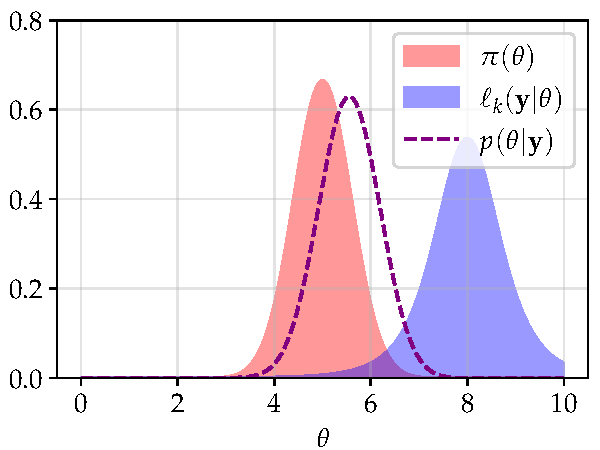
\includegraphics[width=5cm]{figures/intro/posterior1.pdf}
    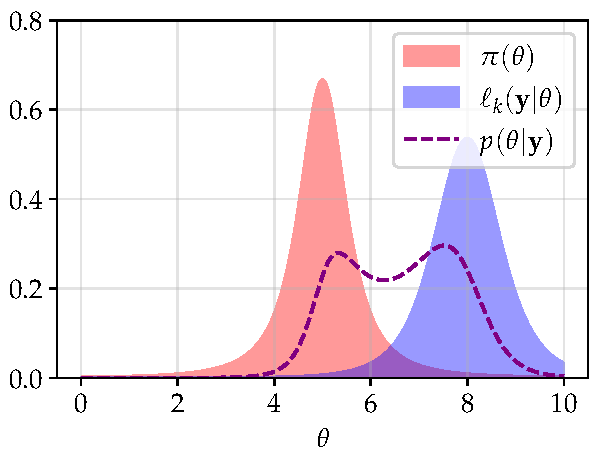
\includegraphics[width=5cm]{figures/intro/posterior2.pdf}
    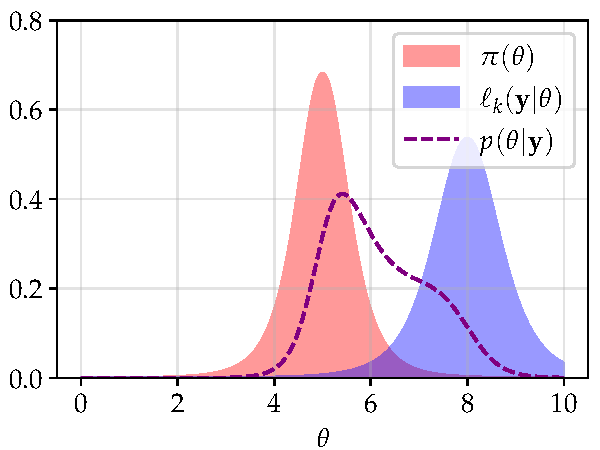
\includegraphics[width=5cm]{figures/intro/posterior3.pdf}   
    \caption{Différents calculs de posteriors (en pointillé) à partir d'une même vraisemblance (bleu) mais de différents priors (rouge).%De gauche à droite le prior est : une gaussienne $\cN(5,)}
    }
    \label{fig:intro-differentsposteriors}
\end{figure}


%On peut déduire d'un tel exemple que les queue de distribution repésente une information décisive au sein d'un prior. Cela illustre 

La question de la construction du prior reste une question ouverte dans la littérature. %tout le worflow bayésien \citep{gelman_bayesian_2020}, elle oppose souvent deux répons%es possibles
%Elle oppose souvent deux axes de refléxions : la définiton de p
Pour certains, elle est l'opportunité d'ajouter de l'information provenant d'une source extérieure, il peut s'agir d'un jugement d'expert, de données historiques, ou de connaissances sur certaines propriétés attendues du résultat. Leurs priors sont plutôt qualifiés d'informatifs.
Pour d'autres, elle est au contraire le moyen d'introduire une incertitude dans le modèle, l'\emph{a priori} est alors dans un tel cas une absence de connaissance, qui vient laisser l'information provenir essentiellement des données. Ces derniers ont confiance en la modélisation de la vraisemblance, et leur prior sera qualifié de non-informatif.


On comprend au travers de ces paragraphes introductifs que cette question est insoluble : il ne peut pas exister de méthode unanime de sélection de prior. Elle illustre même l'un des ``trous'' du workflow bayésien selon \citet{gelman_holes_2020} : les priors trop informés ne permettent pas d'avoir confiance en le moindre résultat tandis que les priors trop peu informés %n'exerguent que trop peu d'estimation crédible.
donnent lieu a des zones de crédibilité parfois trop larges et inutilisables.
%Il ne s'agit pas de décrédibiliser le bayésien 
Ce n'est pas pour autant que l'approche bayésienne perde de son intérêt et cette section n'est pas vouée à discréditer la démarche, la suite du manuscrit le prouvera. %Comme toute méthode elle doit être construite 
Mais elle doit laisser celui ou celle qui l'emploie conscient ou consciente des impacts et des limites de ses choix. Le choix d'un prior est aussi critique que le choix du modèle lui-même.








%Lorsque l'on observe plusieurs réalisations de $Y$ sont observées : $(Y_1,\dots,Y_k)$






\subsection{Ce qui motive la recherche sur l'élicitation de priors pour les études sismiques probabilistes de sûreté}

L'analyse bayésienne a gagné en popularité dans de nombreux domaines, y compris dans des études de fiabilité ou de sûreté. 
En effet, elle est plébiscitée pour sa capacité (i) à introduire et propager une incertitude dans un problème d'inférence, et (ii) à être plus régulière que beaucoup de méthodes fréquentistes, en particulier lorsque le nombre de données observées est limité.

Le cadre de l'inférence bayésienne s'introduit en effet bien dans la démarche de quantification d'incertitu\-des. 
L'identification des incertitudes sur l'entrée $\mbf X$ ou sur le modèle même $\cM$ (ou bien s'il y a lieu le méta-modèle) peut se faire au travers d'une paramétrisation de celles-ci, en donnant lieu à une distribution paramétrique de $Y$ : $\PP_{Y|\mbf X,\theta}$.
La variable $\theta$, aléatoire sous le paradigme bayésien, peut alors représenter diverses sources d'incertitudes, de différentes natures selon les cas \citep{bousquet_contributions_2024}. Cette approche a été employée à pléthore dans divers types de modèles, on peut citer par exemple les cas des processus gaussiens (par ex. \cite{gu_parallel_2016}) ou des réseaux de neurones \citep{arbel_bayes_2023}. 



Parfois, certaines études adoptent la démarche pour la possibilité qu'elle offre d'introduire un jugement  ou une connaissance \emph{a priori}.
C'est pourtant ce même point qui fait aussi débat puisqu'il est la potentielle source d'une subjectivité difficile à justifier.
Dans le cadre des études sismiques probabilistes de sûreté en industrie nucléaire, la démonstration de robustesse est centrale. Les cas d'études y étant souvent très complexes, on trouvera alors parfois autant de priors qu'il y a d'experts en suivant cette démarche.
De tels cas caricaturaux mettent en péril l'auditabilité de la moindre région de crédibilité \emph{a posteriori}.

%De fait, il est essentiel de se chercher à se prévaloir 
%De telles études, compatibles et 
%nécessite l'apport d'un cadre méthodique et rigoureux de 

On comprend en fait que dans une étude de sûreté qui se veut auditable, une ``bonne'' région de crédibilité sur un paramètre estimé n'est pas une région nécessairement étroite, même si elle suggère que la sûreté est satisfaite. A l'inverse, une région trop large n'est pas pour autant ``bonne'' car elle ne permet pas de démontrer la robustesse attendue de l'équipement. L'équilibre est complexe, et le ``bon'' prior est celui qui, bien que démontrant au mieux la capacité ou l'incapacité de l'équipement à résister à l'aléa, produit un résultat inspirant confiance. %Il doit être assuré qu'il est affranchi de l'introduction d

Toutes ces réflexions mettent en lumière l'intérêt d'une construction méthodique du prior dans le cadre des études sismiques probabilistes de sûreté, au travers d'un cadre rigoureux qui vise à éviter, dans la mesure du possible,  l'introduction de la moindre subjectivité dans la démarche.










\section{Esquisse du manuscrit et contributions}

\subsection{Problématiques et plan}

% \subsubsection{Problématiques}


Plusieurs questions principales se détachent de cette introduction et de ces premières réflexions. Elles sont listées ci-dessous, et décrivent les problématiques majeures qui se sont manifestées au cours de cette thèse et auxquelles les travaux présentés dans ce manuscrit cherchent à répondre.\\[-1pt]


\ques{i}{Comment peut-on définir et appuyer l'objectivité d'un prior ?\\ }

\ques{ii}{Quelles sont les limites de l'emploi d'un tel prior, peu informatif par essence, et comment concilier son usage avec les besoins pratiques ?}

\ques{iii}{Comment construire et implémenter de tels priors dans un cas pratique ?\\ }

\ques{iv}{Dans le contexte des études sismiques probabilistes de sûreté, comment s'implémentent ces priors objectifs dans un modèle concret d'estimation de fiabilité sismique ?}

\ques{v}{Quelles conséquences peut avoir le manque d'information \emph{a priori} ou provenant des données dans ce modèle et comment les solutionner ?}

\ques{vi}{Comment peut-on bénéficier au mieux des différentes sources d'information (celle \emph{a prirori} et celle issue des données) dans le workflow bayésien du modèle étudié dans son ensemble ?}\\


Dans cette thèse, nous tentons de répondre à ces six problématiques au travers d'une étude selon deux axes. Le premier axe a une dimension qualifiée de théorique, en adressant les problématiques liées à la construction de prior dits ``objectifs'' dans son ensemble. Il se concentre sur le développement d'une théorie appelée la théorie des priors de référence. Le second axe est alors plutôt qualifié de pratique, en étudiant la mise en œuvre des développements théoriques sur des cas d'études réels, en se concentrant sur l'estimation de courbes de fragilité sismique, qui représentent un outil important du cadre des études sismiques probabilistes de sûreté.
Il reste important de rappeler que, bien qu'indépendants, les deux grands axes de travail sus-mentionnés s'alimentent l'un l'autre. Ce sont autant les problématiques pratiques qui ont motivé les recherches théoriques, que les découvertes théoriques qui ont été mises au service des études pratiques.\\


%l'un étant plutôt théorique et adresse les questions de construction, de définiton, et d'objectivité des priors ; l'autre étant plut
% Ainsi, la premère partie de ce manuscrit est 




La \textbf{\cref{part:ref-theory}} de ce manuscrit est alors dévouée au développement de la théorie des priors de référence.

\noindent
Dans le \cref{chap:intro-ref}, on introduit la théorie et on développe son état de l'art. Il permet d'introduire la notion de prior de référence telle qu'elle est communément définie dans la littérature, et sa place parmi les priors objectifs. Ce chapitre permet aussi de formaliser le cadre mathématique de travail pour la suite de la partie.

\noindent
Dans le \cref{chap:ref-generalized}, on observe que la définition des priors de référence s'appuie sur une mesure de dissimilarité. On cherche alors dans ce chapitre à généraliser la définition de cette dernière afin d'appuyer le caractère objectif des priors de référence. Ce chapitre apporte une réponse à la \textbf{question i}.

\noindent
Dans le \cref{chap:constrained-prior}, on cherche une ouverture au cadre des priors de référence, lorsqu'il donne lieu à des priors difficilement utilisables en pratique. On propose alors une définition de ce qu'on appelle priors de référence contraints. Les solutions de cette définition apportent une réponse à la \textbf{question ii}.

\noindent
Dans le \cref{chap:varp}, on développe une méthode numérique d'approximation des priors de référence. Cette méthode s'appuie sur l'inférence variationnelle en définissant le prior comme la sortie d'un réseau de neurones, afin d'éviter un calcul explicite de celui-ci. Ce chapitre apporte une réponse à la \textbf{question iii}. \\


La \textbf{\cref{part:spra}} de ce manuscrit aborde le sujet de l'estimation bayésienne dite objective des courbes de fragilité sismique.

\noindent
Dans le \cref{chap:frags-intro}, on introduit les courbes de fragilité sismique, leur définition, leur historique et leur intégration dans le cadre des études sismiques probabilistes de sûreté. Un état de l'art des méthodes d'estima\-tion de ces courbes suivant les différents types de données à disposition y est proposé.

\noindent
Dans le \cref{chap:prem}, on propose un calcul et une étude en profondeur du prior de référence pour un modèle classique employé pour l'estimation de ces courbes de fragilité. L'inférence bayésienne via l'emploi de ce prior y est comparée à d'autres méthodes. Ce chapitre apporte une réponse à la \textbf{question iv}.

\noindent
Dans le \cref{chap:constrained-frags}, on s'intéresse en profondeur aux limites du modèle considéré pour l'estimation des courbes de fragilité. On propose une solution qui est appuyée par les développements théoriques de la première partie. Ce chapitre apporte une réponse à la \textbf{question v}.

\noindent
Dans le \cref{chap:doe}, on termine notre étude en proposant une méthode qui vient appuyer l'estimation bayésienne en optimisant l'information issue des données non plus seulement  lors du choix du prior mais également lors de la sélection de celles-ci, au travers d'une méthode de planification d'expériences. Ce chapitre apporte une réponse à la \textbf{question vi}.\\


Une conclusion générale viendra clore le manuscrit dans une \textbf{\cref{part:conclusion}} finale.


\subsection{Liste des contributions}

La recherche conduite au cours de cette thèse a donné lieu à plusieurs contributions dans la littérature scientifique. Ci-après sont listés les travaux publiés et soumis pendant celle-ci.

\nocite{van_biesbroeck_design_2025,van_biesbroeck_generalized_2024,van_biesbroeck_influence_2023,van_biesbroeck_properly_2024,van_biesbroeck_reference_2024,baillie_variational_2025,baillie_bayesian_2025,van_biesbroeck_design_2025-1}


\subsubsection{Articles de revues}

\begin{itemize}
    \item \textbf{A. Van Biesbroeck}, C. Gauchy, C. Feau \& J. Garnier (2025). ``Robust a posteriori estimation of probit-lognormal seismic fragility curves via sequential design of experiments and constrained reference prior''. \emph{arXiv} 2503.07343. \textsc{doi:} \href{https://dx.doi.org/10.48550/arXiv.2503.07343}{10.48550/arXiv.2503.07343}.
    \item N. Baillie, \textbf{A. Van Biesbroeck} \& C. Gauchy (2025). ``Variational inference for approximate reference priors using neural networks''. \emph{arXiv} 2502.02364. \textsc{doi:} \href{https://dx.doi.org/10.48550/arXiv.2502.02364}{10.48550/arXiv.2502.02364}
    \item \textbf{A. Van Biesbroeck} (2024). ``Properly constrained reference priors decay rates for efficient and robust posterior inference'', \emph{arXiv} 2409.13041. \textsc{doi:} \href{https://dx.doi.org/10.48550/arXiv.2409.13041}{10.48550/arXiv.2409.13041}
    \item \textbf{A. Van Biesbroeck}, C. Gauchy, C. Feau \& J. Garnier (2025). ``Design of experiments based on a low fidelity model for seismic fragility curves estimation''. \emph{ESAIM: ProcS} (to appear). \textsc{hal:} \href{https://hal.science/hal-04719458v1}{hal-04719458v1}
    \item \textbf{A. Van Biesbroeck} (2023). ``Generalized mutual information and their reference priors under Csizar f-divergence''. \emph{arXiv} 2310.10530. \textsc{doi:} \href{https://dx.doi.org/10.48550/arXiv.2310.10530}{10.48550/arXiv.2310.10530}
    \item \textbf{A. Van Biesbroeck}, C. Gauchy, C. Feau \& J. Garnier (2024). ``Reference prior for Bayesian estimation of seismic fragility curves''. \emph{Probabilistic Engineering Mechanics}, 76, pp 103622. \textsc{doi:} \href{https://dx.doi.org/10.1016/j.probengmech.2024.103622}{10.1016/j.probengm\-ech.2024.103622}
\end{itemize}



\subsubsection{Articles de conférences}

\begin{itemize}
    \item \textbf{A. Van Biesbroeck}, C. Feau \& J. Garnier (2025). ``Design of experiments for efficient and conform Bayesian learning of seismic fragility curves''. \emph{Proceedings of the 28th conference on Structural Mechanics in Reactor Techology (SMiRT).}
    \item N. Baillie, \textbf{A. Van Biesbroeck}, C. Feau \& C. Gauchy (2025). ``Bayesian estimation of seismic fragility curves based on variational reference priors using neural networks''. \emph{Proceedings of the 6th Thematic Conference on Uncertainty Quantification in Computational Sciences and Engineering (UNCECOMP)}.
    % \item C. Gauchy, \textbf{A. Van Biesbroeck}, C. Feau \& J. Garnier (2023). ``Inférence variationelle de lois a priori de référence''. \emph{Proceedings des 54èmes Journées de Statistiques (JdS)}. \textsc{url}
    \item \textbf{A. Van Biesbroeck}, C. Gauchy, J. Garnier \& C. Feau (2023). ``Connections between reference prior theory and global sensitivity analysis, an illustration with f-divergences''. \emph{Proceedings des 54èmes Journées de Statistiques (JdS)}. \textsc{hal:} \href{https://hal.science/hal-04171446}{hal-04171446}
    \item \textbf{A. Van Biesbroeck}, C. Gauchy, C. Feau \& J. Garnier (2023). ``Influence of the choice of the seismic intensity measure on fragility curves estimation in a Bayesian framework based on reference prior''. \emph{Proceedings of the 5th Thematic Conference on Uncertainty Quantification in Computational Sciences and Engineering (UNCECOMP)}, pp. 94-111. \textsc{doi:} \href{https://dx.doi.org/10.7712/120223.10327.19899}{10.7712/120223.10327.19899}
\end{itemize}


Chacune de ces publications, qu'elle prenne la forme d'un article de journal ou de conférence propose une contribution originale et liée à cette thèse. Naturellement, les contributions présentées dans des articles de revues sont considérées comme plus percutantes.

Mis à part deux exceptions, chacune de ces contributions se voit au centre d'un chapitre ou d'une annexe de ce manuscrit.
La première exception est l'article de conférence publié aux JdS de 2023. En effet ce travail a constitué une introduction à l'étude qui a donné lieu plus tard à l'article de revue intitulé ``Generalized mutual information and their reference priors under Csizar f-divergence''. Dans cette thèse, l'article de conférence est donc incorporé au chapitre lié à ce dernier papier de revue (\cref{chap:ref-generalized}).
La seconde exception est l'article de conférence publié à SMiRT en 2025. La méthodologie originale proposée dans cet article reste conceptuelle et s'est heurtée au calendrier de fin de thèse. %Un approfondissement qui pourrait lui être apporté dans le futur saurait 
Elle manque alors d'un approfondissment qui pourrait lui être apporté dans le futur.


%
%
% 
%
% Certaines de ces contributions se retrouvent plutôt dans les chapitres annexes 
% Seule une contribution ne s'illustre pas dans ce manuscrit, il s'agit de l'article de conférence publiée dans les proceedings de SMiRT28.
% Les 


% Chaque publication propose une publication orginale 
% autour de laquelle se contruit 'un des chapitre ou l'une des annexes de ce manuscrit.
%bien que les constributions présentées en tant qu'articles de journaux sont naturelemnt plus importantes.



%qui se retrouv. 



















%Pour répondre à ces problématiques, 



  % What are the ways to define objectively a prior? Are they totally objective? Are the objective priors the most intersting priors to consider, or should we discriminate judiciously some class of priors? How to compute and implement the objective priors? 
    % What does they look like in the context of SPRA? How to use them in that context and what are the obstacles of the Bayesian approach in the context? 










\newpage
\thispagestyle{plain}
\renewcommand{\chaptertitlenamelng}{Chapter}
\renewcommand{\partname}{Part}